\section {Tactile attention and memory in multi-finger contact}
People often use several digits simultaneously to touch surfaces. Thus, they may use two fingers (eg index and middle) side by side (e.g. in steadying themselves against a stable surface) or they might use thumb opposing the index (and possibly other fingers) to form a precision grasp on either side of an object (e.g. stair rail). Often the surfaces contacted by the two digits will be the same and the double contact affords improved tactile sensitivity over single contact. However, two surfaces that are not co-located may differ in texture. For example, when using precision grip to feel fabric, the “front” and “back” surfaces may have very different textures. The perceived texture of either surface is then likely to be affected by the surface on the reverse side. We have been investigating such contact in terms of interactive effects on roughness judgments arising from simultaneous contact with two separate surfaces. Depending on the two digits involved, we have shown attention and neural cross talk afford explanations of some of the effects seen \cite{roberts2010, roberts2013}. Within CoDyCo we have been contrasting two forms of perceptual judgment, based on single (magnitude estimation) and two successive presentations (2-interval forced choice) of the surfaces. The theoretical interest is in the potential role of short term tactile memory in the second case. Similarity of the two digit judgments despite differences in working memory requirements in the different perceptual tasks inclines us against a significant role for a memory component in multi-digit roughness perception. A paper is in preparation on this topic. 

\begin{figure}
  \centering
  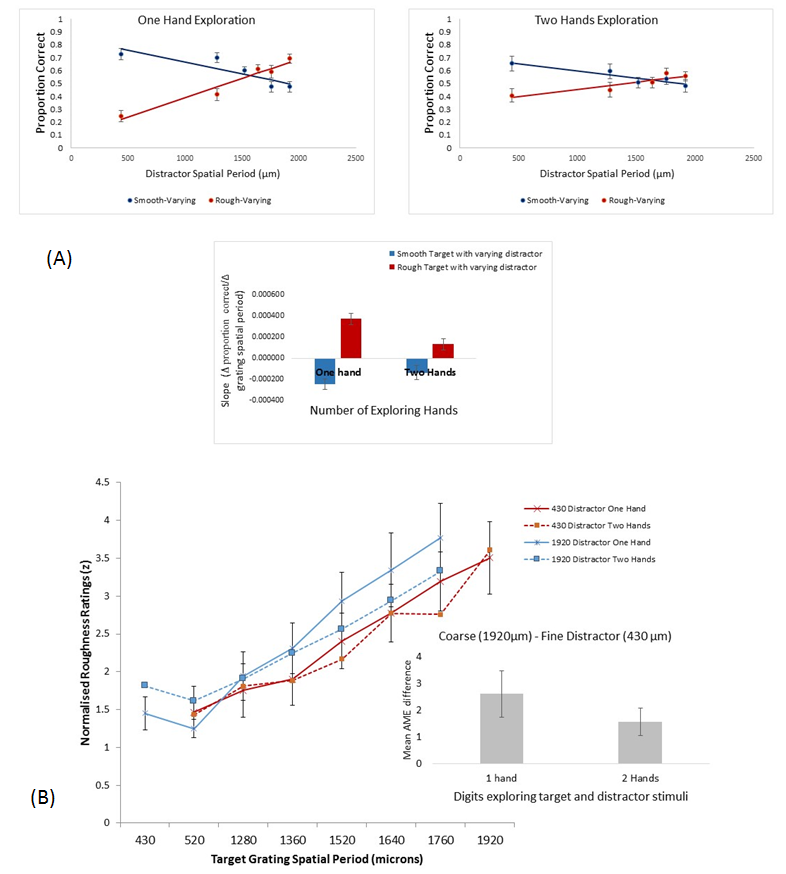
\includegraphics[width=.7\textwidth]{Roberta/Figures/Figure1.png}
  \caption{Multifinger contact effects on (A, above) 2-interval force choice (2-IFC) and (B, below) absolute magnitude estimates (AME) measures of roughness perception. In both tasks participants actively explored a target and distractor surface simultaneously using 2 digits; the digits were either on one hand or two hands, expected to result in more or less crosstalk. In the 2-IFC task (A), participants identified the rougher of a pair of target stimuli and were instructed to ignore the distracter. The red circles and line indicate group (N=12) average performance when the fine surfaced target was paired with various coarse distractor surfaces; a fine distractor depresses accuracy more than a coarse distractor. The blue circles and line show behaviour with the coarse target; a coarse distractor depresses accuracy more than does a fine one. The bar graph summarising mean slope across participants shows the distraction effect is greater in the one hand condition. 
In the AME task (B), participants rated the roughness of target surfaces while instructed to ignore the simultaneously touched distractor. The graph at the top of figure 1b shows mean ratings for each target surface. The blue crosses and squares show mean ratings for each target surface with a coarse distractor surface. Mean ratings with a fine distractor surface are shown in red. It can be seen that a coarse distracter results in higher roughness ratings than does a fine distracter. As with 2-IFC, the distracter effects are greater with the distracter on the same hand as the target.}
  \label{Multifingercontacts}
\end{figure}

\section {Surface roughness effects on brain activation in static and sliding contact}
Duplex theory proposes that surface roughness judgments are mediated by a combination of vibratory and spatial inputs from the slowly and rapidly adapting tactile mechanoreceptors \cite{Hollins2000}. Tactile processing by the brain primarily involves the somatosensory cortex. However, cortical areas primarily associated with auditory and visual input can also be involved. Thus, recently it has been shown that direct current stimulation of the visual or auditory cortex can facilitate spatial or temporal tactile judgments \cite{yau2014}. We are currently completing a brain imaging study in which we expect to demonstrate a neural basis for duplex theory. Thus we expect moving sliding textures will activate auditory cortex while static coarse textures invoke visual cortex; preliminary data in Figure 2 show auditory cortex activation with sliding contact.
 
\begin{figure}[!h]
  \centering
  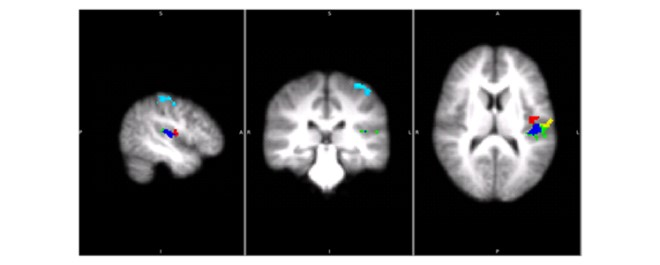
\includegraphics[width=.7\textwidth]{Roberta/Figures/Figure2.jpg}
  \caption{Activations during passive touch.  The three panels indicate sagittal, coronal and horizontal planar sections of the brain with multisensory activations for a tactile discrimination task contrasting coarse and fine texture perception under moving and static touch conditions. Regions of interest shown with coloured blobs, were more activated for moving (vs static) touch, including auditory cortex (TE1.0). The stimuli were applied to the right index finger of passive participants, N=13; Light blue: BA1, Green: OP1, Red: OP3, Yellow: OP4, Blue: TE1.0}
  \label{Activations during passive touch}
\end{figure}

\section {The role of uncertainty in shared control of grip in cooperative lifting}
Social processes in cooperative multi-person action is a major topic in psychology, but there has been very little analysis of kinematics and dynamics of joint action. We have been examining control of precision grip force during a 2-person lifting task in which the load to be lifted varies from trial to trial. There are three conditions that manipulate load uncertainty. In the first condition the weight is unknown to either participant. In the second condition it is known to just one of the participants, while in the third condition it is known to both of them.  We find systematic changes in anticipatory grip as a function of both one’s own knowledge but also what is known by one’s partner (see Figure 3).

\begin{figure}[!h]
  \centering
  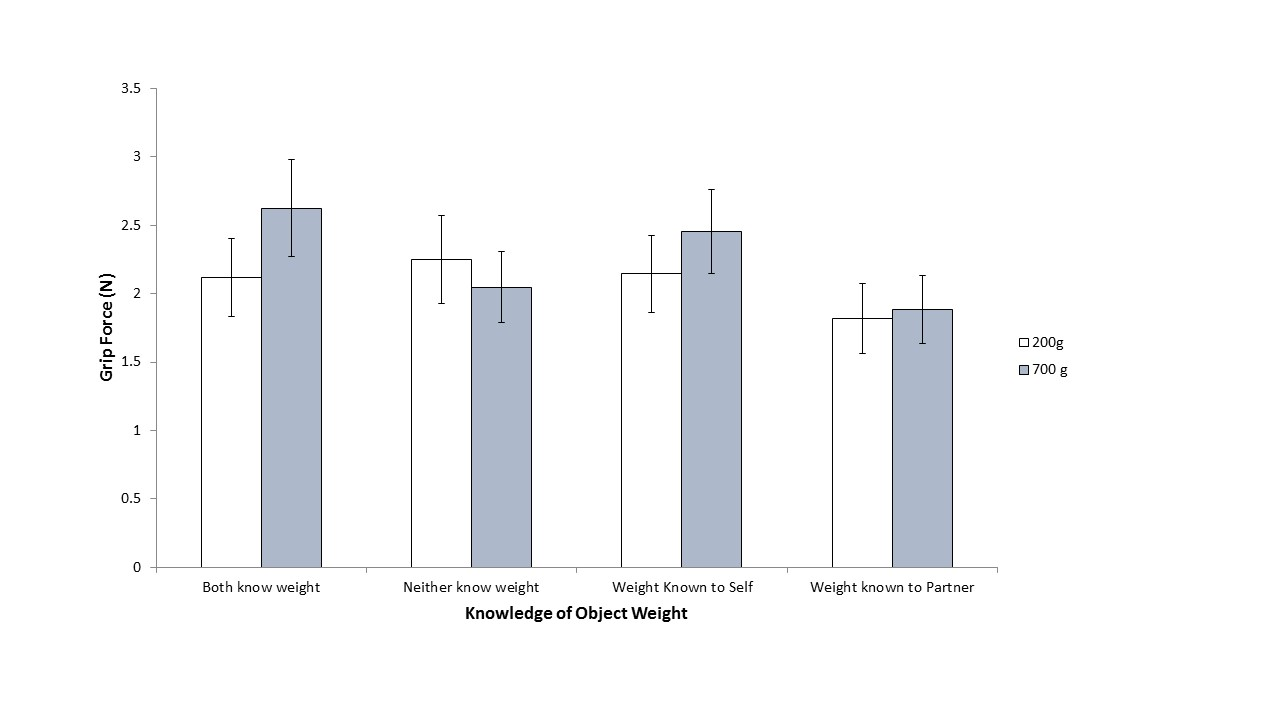
\includegraphics[width=.8\textwidth]{Roberta/Figures/Figure3.jpg}
  \caption{Joint lifting action. The participants worked in pairs to lift a bar to a target height. The weight at the centre of the bar (either 200g or 700g) was known to one, both or neither participant in pair. The force with which the participants held the bar in anticipation of a lift in the different knowledge conditions is shown along with on SE of the mean.}
  \label{Joint lifting action}
\end{figure}
